\begin{tikzpicture}
\tikzset{other/.style={dashed, draw=blue, fill=blue, fill opacity=0.1, text opacity=1, text=black}}
\tikzset{focus/.style={dashed, draw=red, fill=red, fill opacity=0.1, text opacity=1, text=black}}
\tikzset{outside/.style={dashed, draw=gray, fill=gray, fill opacity=0.1, text opacity=1, text=gray}}

\coordinate (O) at (0,0) ;
\coordinate (A) at (10,0) ;
\coordinate (B) at (0,10) ;

\only<9>{
\filldraw [focus] (6.5,3) ellipse (2 and 1) node[scale = 1] (L) {$L$};
}

\only<1->{
\filldraw [other] (2,1) circle (1) node[scale = 1] (CTT) {$CTT$};
}

\only<2->{
\filldraw [other] (9,6) ellipse (1 and 3) node[scale = 1] (BM)  {$B$};
}

\only<3->{
\filldraw [other] (6,6) ellipse (1 and 2) node[scale = 1] (ICO)  {$ICO$};
}

\only<4->{
\filldraw [other] (3.5,4) ellipse (2 and 1) node[scale = 1] (EOFM)  {$EOFM$};
}

\only<5->{
\filldraw [other] (7.5,5.5) ellipse (1 and 2) node[scale = 1] (Istar)  {$Istar$};
}

\only<6->{
\filldraw [other] (7,8.5)  ellipse (1 and 1.5) node[scale = 1] (SD)  {$SD$};
}

\only<7->{
\filldraw [outside] (1,8) ellipse (1 and 2) node[scale = 1, text width=2cm, text centered] (NeuroScience) {$Sciences$ $Cognitives$};
}

\only<8->{
\filldraw [outside] (9,9) ellipse (1 and 1) node[scale = 1] (Codage) {$Codage$};
}


%% axis :
\draw [->][>=latex] (O) -- (A);
\draw [->][>=latex] (O) -- (B);
\draw (A) node [below] {$Machine$};
\draw (O) node [below] {$Homme$};
\draw (B) node [left] {$Concret$};
\draw (O) node [left] {$Abstrait$};
\end{tikzpicture}
